%Définir le format du document: papier, taille de police, type de document, etc.
%La mise en page du rapport, NE PAS MODIFIER.
\documentclass[11pt, french]{article}

%%%%%%%%%% Packages externes utilisés %%%%%%%%%%%%%%%%%%%
\usepackage[french]{babel}
\selectlanguage{french}
\usepackage[T1]{fontenc}
\usepackage[utf8]{inputenc}

\usepackage{verbatim}
\usepackage{graphicx}
\usepackage{epstopdf}
\usepackage{macro}
\usepackage{url}
\usepackage{algorithm}
\usepackage{algorithmic}
%\usepackage{algorithm2e}

%La mise en page du rapport, NE PAS MODIFIER.
\usepackage{geometry}
 \geometry{
 a4paper,
 left=20mm,
 right=20mm,
 top=20mm,
 bottom=20mm,
 }

%%%%%%%%% Le corps du document entre begin et end %%%%%%%%%%%%%%%%%%%
\begin{document}

%Page de garde
%%%%%%%%%%%%%%% Page de garde %%%%%%%%%%%%%%%%%%%

\begin{titlepage}
    \begin{center}
        \vspace*{20mm}
        
        {\Large \textbf{CY Cergy Paris Université}}
        
        \vspace*{5mm}
        {\large \textbf{Département Informatique}}
        
        \vspace*{15mm}
        
        {\Large \textbf{RAPPORT DE PROJET}}
        
        \vspace*{3mm}
        {\large Génie Logiciel - L2 Informatique}
        
        \vspace*{3mm}
        {\large Année universitaire 2025-2026}
        
        \vspace*{20mm}
        
        \rule{0.8\textwidth}{1pt}
        \vspace*{5mm}
        
        {\Huge \textbf{Jeux de carte à joueur multiple :}} \\
        \vspace*{5mm}
        {\Huge \textbf{``Tu n'y peux rien''}}
        
        \vspace*{5mm}
        \rule{0.6\textwidth}{1pt}
        
        \vspace*{15mm}
        
        \begin{tabular}{r l}
            \textbf{Encadré par :} & M. Tianxiao LIU \\
            \textbf{Rédigé par :}  & KHODJA Laiza \\
                                   & BOUATMANE Nesrine \\
                                   & BERRANDOU Nassim \\
        \end{tabular}
        
        \vspace*{15mm}
        
        \rule{0.8\textwidth}{0.5pt}
        
        \vspace*{10mm}
        
        {\large Avril 2026}
        
        \vspace*{10mm}
        
        
\includegraphics[width=6cm]{images/cy-logo.png}
        
    \end{center}
\end{titlepage}


%Génération automatique de la table des matières, de la liste des figures et de la liste des tableaux
\tableofcontents
\listoffigures
\listoftables


\newpage
\section* {Remerciements}
\addcontentsline{toc}{section}{Remerciements}
Les auteurs du projet voudraient remercier vivement :

\begin{itemize}
\item M. Tianxiao LIU, enseignant du module Génie Logiciel, pour ses conseils et son accompagnement tout au long du projet.
\item CY Cergy Paris Université pour nous avoir fourni les ressources nécessaires à la réalisation de ce travail.
\item L'équipe pédagogique de la Licence Informatique pour la qualité de la formation.
\end{itemize}

\newpage
\section{Introduction}
\label{sec:introduction}

\subsection{Contexte du projet}
\paragraph{} Le projet "Tu n'y peux rien" s'inscrit dans le cadre de l'UE Génie Logiciel de deuxième année à CY Cergy Paris Université. L'objectif est de développer un jeu de cartes multijoueur en Java, respectant des règles spécifiques et intégrant des bots de différents niveaux de difficulté.

\paragraph{} Ce projet s'inscrit dans la continuité des enseignements de programmation orientée objet et de génie logiciel. Il mobilise des compétences variées : conception UML, développement Java, gestion de projet avec Git, tests unitaires et documentation.

\subsection{État de l'art des jeux de cartes}
\paragraph{} Les jeux de cartes occupent une place importante dans l'histoire du jeu vidéo. Des titres comme \textit{Uno}, \textit{Skip-Bo} ou \textit{7 Wonders} proposent des mécaniques basées sur l'enchère et la pose de combinaisons. Cependant, peu de jeux intègrent une règle de "carte 2 écrase tout" ni un système de bombes et jokers comme dans notre projet.

\paragraph{} Le jeu "Tu n'y peux rien" se distingue par plusieurs originalités. Tout d'abord, la carte 2 possède un statut particulier : elle écrase toute carte simple posée précédemment. Ensuite, les Jokers sont polymorphes : ils peuvent remplacer n'importe quelle carte manquante dans une combinaison. Enfin, trois niveaux de difficulté pour les bots offrent une expérience de jeu adaptée à tous les publics.

\subsection{Objectif du projet}
\paragraph{} Recréer ce jeu de cartes au format numérique où un joueur humain affronte 2 à 4 bots. Le jeu doit gérer les combinaisons (simple, double, série, bombe, double joker), les cartes spéciales (2, Joker), et calculer les scores en fin de partie. L'interface graphique doit être intuitive et responsive, avec un design soigné (thème casino).

\subsection{Organisation du rapport}
\paragraph{} La section \ref{sec:specification} présente le cahier des charges et les fonctionnalités attendues. La section \ref{sec:conception} détaille la conception du logiciel et la section \ref{sec:oeuvre} présente sa mise en œuvre. La section \ref{sec:manuel} est un manuel utilisateur. La section \ref{sec:deroulement} décrit le déroulement du projet. La section \ref{sec:conclusion} conclut et propose des améliorations.

\newpage
\section{Spécification du projet}
\label{sec:specification}

\subsection{Notions de base et contraintes du projet}
\label{sec:spec1}

\paragraph{Fonctionnement général du logiciel}
Le jeu se déroule en tours. Chaque joueur reçoit 5 cartes au début. 
Le joueur avec la plus petite carte (hors 2 et Joker) commence. 
À chaque tour, le joueur doit poser une combinaison qui bat la précédente. 
Si aucun joueur ne peut jouer, le tas est réinitialisé.

\paragraph{Déroulement détaillé d'une partie}
Une partie se décompose en plusieurs rounds. Chaque round permet à chaque joueur de jouer à tour de rôle. Lorsqu'un joueur ne peut pas jouer, il pioche une carte et passe son tour. Si tous les joueurs passent leur tour sans jouer (sauf le dernier ayant joué), le tas est réinitialisé : toutes les cartes sont mélangées et replacées dans la pioche. La partie se termine immédiatement lorsqu'un joueur pose sa dernière carte.

\paragraph{Notions et terminologies de base}
\begin{itemize}
\item \textbf{Carte} : 54 cartes (52 standards + 2 Jokers). Les valeurs vont du 2 à l'As.
\item \textbf{Combinaison simple} : 1 carte. C'est la combinaison la plus élémentaire.
\item \textbf{Double} : 2 cartes de valeur identique (exemple : deux Rois).
\item \textbf{Série} : 3 cartes ou plus dont les valeurs se suivent (exemple : 4,5,6).
\item \textbf{Bombe} : 3 ou 4 cartes de valeur identique. Une bombe bat toute combinaison simple.
\item \textbf{Double Joker} : 2 Jokers ensemble. C'est la combinaison la plus puissante.
\end{itemize}

\paragraph{Hiérarchie des combinaisons}
Les combinaisons sont classées par force croissante : Simple (<) Double (<) Série (<) Bombe (<) Double Joker. Une combinaison ne peut battre une autre que si elle est de force supérieure ou égale (cas des séries où les cartes doivent être plus hautes).

\paragraph{Contraintes et limitations connues}
\begin{itemize}
\item Langage : Java 8 (compatibilité ascendante)
\item Interface graphique : Swing (bibliothèque standard)
\item Bibliothèques externes : Log4j pour les logs, JUnit pour les tests, jFreeChart pour les graphiques
\item Problème connu : la musique ne fonctionne que sous Windows (bug du format WAV sous Linux)
\item L'interface est conçue pour une résolution minimale de 1200x650 pixels
\end{itemize}

\subsection{Fonctionnalités attendues du projet}
\label{sec:spec2}

\paragraph{Fonctionnalités implémentées}
L'ensemble des fonctionnalités demandées dans le cahier des charges a été réalisé :
\begin{itemize}
\item Distribution de 5 cartes à chaque joueur en début de partie
\item Détection automatique du joueur qui commence (carte la plus faible)
\item Pose de combinaisons (simple, double, série, bombe, double joker)
\item Gestion des cartes spéciales (2 écrase tout, joker polymorphe)
\item Pioche automatique si aucune carte jouable
\item Reset du tour quand tous les joueurs passent
\item Recyclage du deck quand il est vide
\item Interface graphique complète (menu, options, jeu, fin de partie)
\item 3 niveaux de difficulté pour les bots (Facile, Moyen, Difficile)
\item Système de scores (1 carte = 1 point, bombe = ×2, double joker = ×4)
\item Logs détaillés (format texte et HTML)
\item Tests unitaires JUnit (couverture des classes critiques)
\item Graphiques statistiques avec jFreeChart (camembert et barres)
\end{itemize}

\paragraph{Fonctionnalités non implémentées (hors périmètre)}
Certaines fonctionnalités n'ont pas été retenues dans le périmètre du projet :
\begin{itemize}
\item Mode multijoueur en ligne
\item Sauvegarde des parties
\item Version mobile
\end{itemize}

\newpage
\section{Conception et mise en œuvre}
\label{sec:impl}

\subsection{Architecture globale du logiciel}
\paragraph{} L'architecture du projet suit le modèle MVC (Modèle-Vue-Contrôleur) :

\begin{itemize}
\item \textbf{Modèle (engine.data)} : Classes Card, Deck, Player, GameStats
\item \textbf{Contrôleur (engine.process)} : Classes Game, Combination, BotPlayer
\item \textbf{Vue (gui)} : Classes MainGUI, MenuGUI, OptionGUI, EndGameGUI
\end{itemize}

\begin{figure}[h!]
\centering
%\includegraphics[width=12cm]{images/architecture.png}
\caption{Architecture du logiciel}
\label{fig:architecture}
\end{figure}

\subsection{Classes de données (engine.data)}
\paragraph{}
\begin{itemize}
\item \textbf{Card} : Représente une carte avec sa valeur et sa couleur. Implémente equals() et hashCode().
\item \textbf{Deck} : Gère le paquet de 54 cartes, mélange (shuffle) et pioche (draw).
\item \textbf{Player} : Gère la main du joueur, la pioche et la pose de combinaisons.
\item \textbf{CombinationType} : Énumération des types (SIMPLE, DOUBLE, SERIES, BOMB, DOUBLE\_JOKER, INVALID).
\item \textbf{GameStats} : Enregistre les statistiques et calcule les scores.
\end{itemize}

\subsection{Traitements (engine.process)}
\paragraph{}
\begin{itemize}
\item \textbf{Combination} : Détection automatique du type avec determineType(), comparaison avec canBeat().
\item \textbf{Game} : Logique principale (gestion des tours, pioche, reset, recyclage).
\item \textbf{BotPlayer} : Classe abstraite avec stratégies différentes.
\item \textbf{EasyBot} : Joue aléatoirement, 30\% de chance de passer.
\item \textbf{MediumBot} : Évite les bombes, joue les combinaisons faibles.
\item \textbf{HardBot} : Stratégique, privilégie les combinaisons fortes.
\end{itemize}

\begin{figure}[h!]
\centering
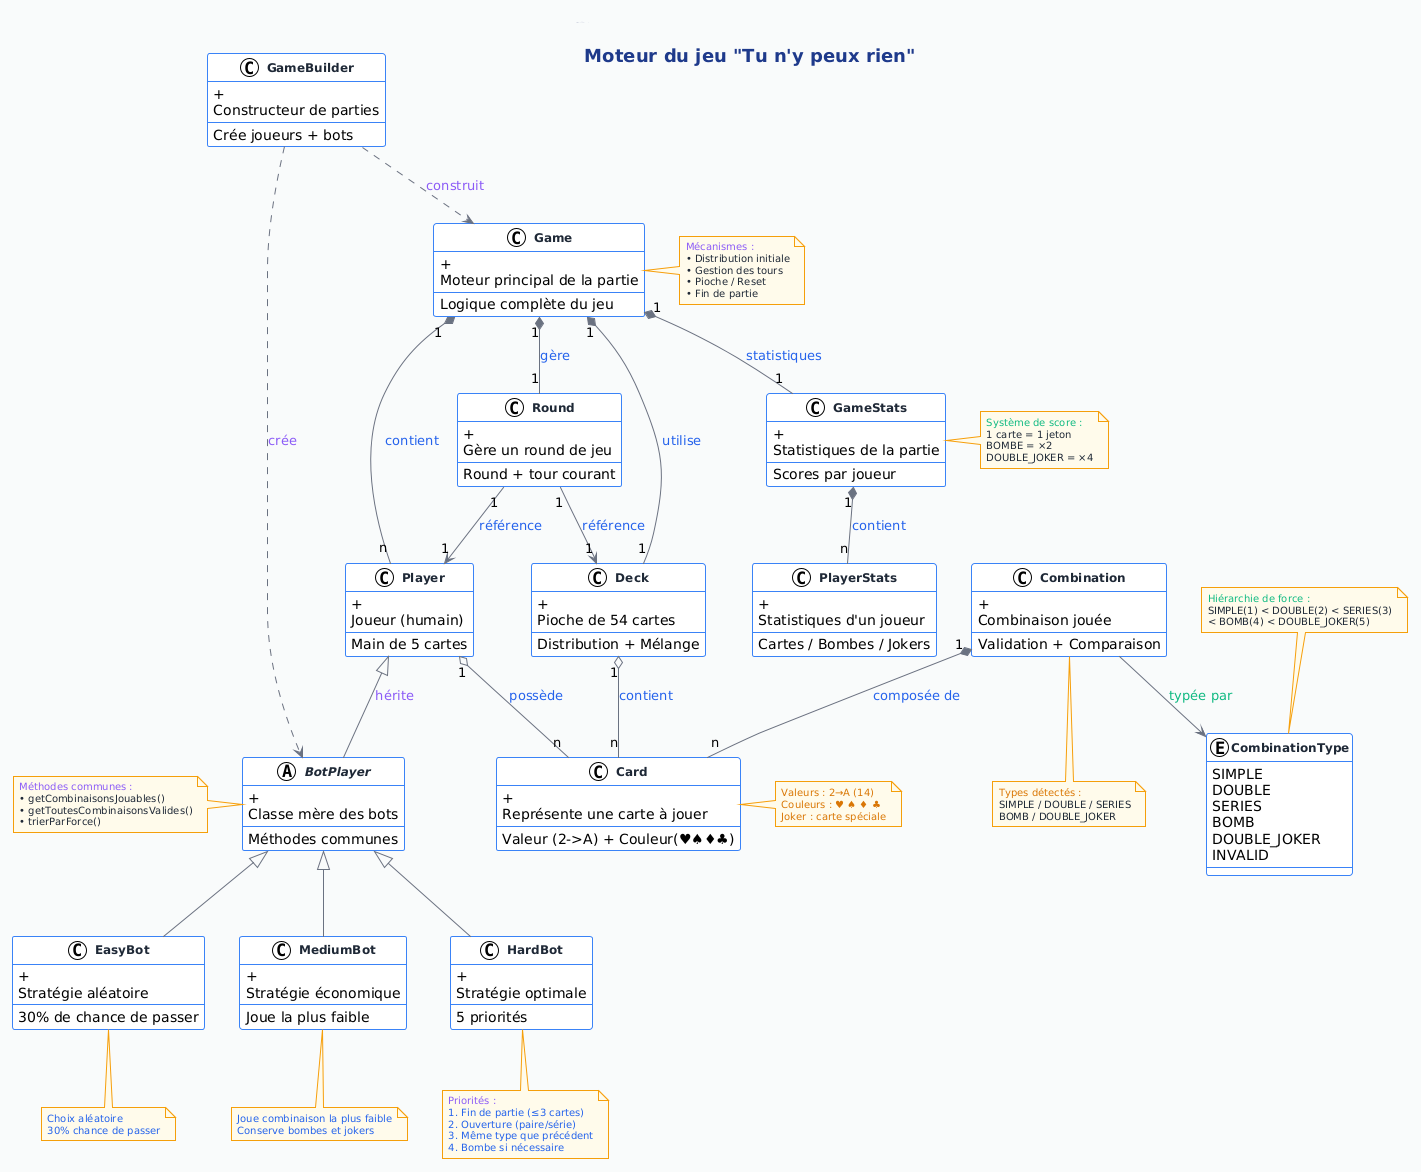
\includegraphics[width=14cm]{images/diagramme_classes.png}
\caption{Diagramme de classes UML}
\label{fig:uml}
\end{figure}

\subsection{IHM Graphique (gui)}
\paragraph{} L'interface est organisée en trois sous-dossiers :

\begin{itemize}
\item \textbf{screens/} : Écrans complets (MainGUI, MenuGUI, OptionGUI, EndGameGUI)
\item \textbf{panels/} : Composants réutilisables (CardPanel, BotsPanel, DeckPanel, GameInfoBar, GameLogPanel)
\item \textbf{utils/} : Utilitaires (GameStyle, CardPaintStrategy, MusicPlayer)
\end{itemize}

\subsection{Patterns de conception utilisés}
\paragraph{}
\begin{itemize}
\item \textbf{Héritage} : BotPlayer → EasyBot, MediumBot, HardBot
\item \textbf{Factory} : GameBuilder.createBot()
\item \textbf{MVC implicite} : Séparation data/process/gui
\item \textbf{Stratégie} : Comportements différents des bots
\item \textbf{Singleton implicite} : GameStyle.isFullscreen
\end{itemize}

\newpage
\section{Manuel utilisateur}
\label{sec:manuel}

\subsection{Lancement du jeu}
\paragraph{} Exécutez la classe \texttt{test.TestGame}. Le menu principal apparaît.

\begin{figure}[h!]
\centering
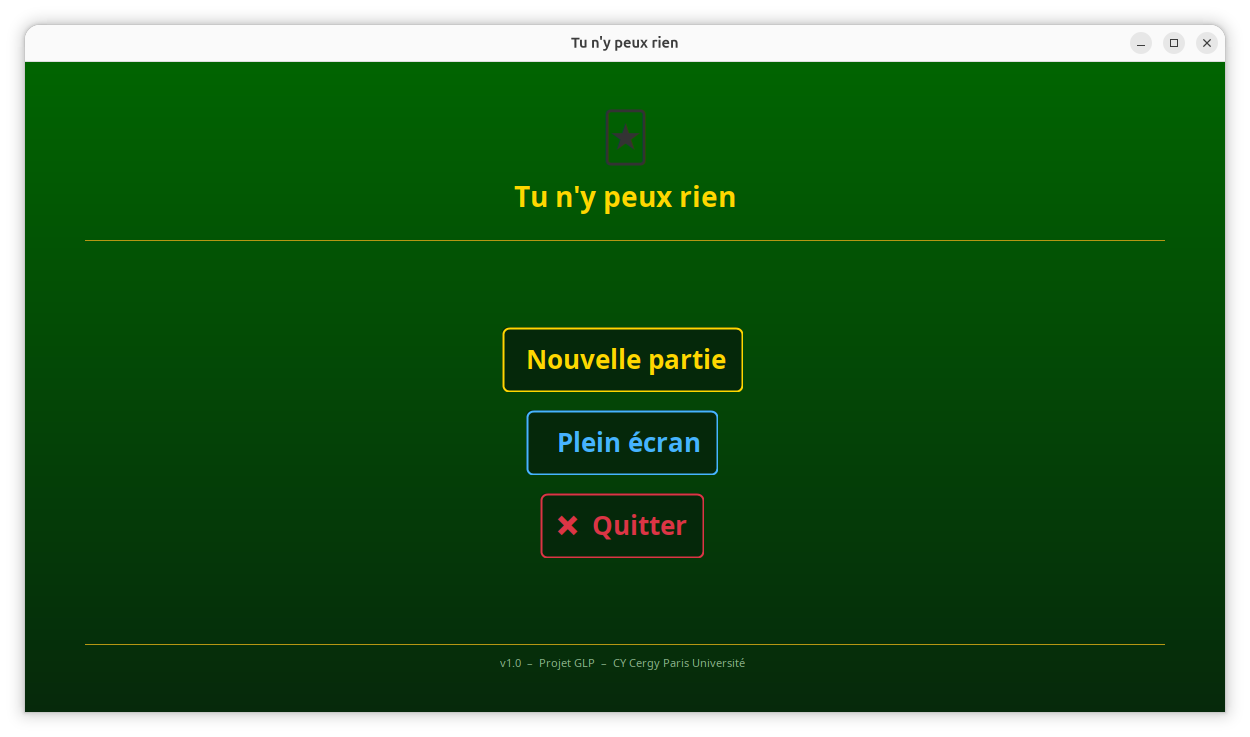
\includegraphics[width=10cm]{images/menu.png}
\caption{Menu principal}
\label{fig:menu}
\end{figure}

\subsection{Configuration de la partie}
\paragraph{} Cliquez sur "Nouvelle partie" pour accéder aux options. Sélectionnez le nombre de joueurs (3 à 5) et la difficulté des bots (Facile, Moyen, Difficile).

\begin{figure}[h!]
\centering
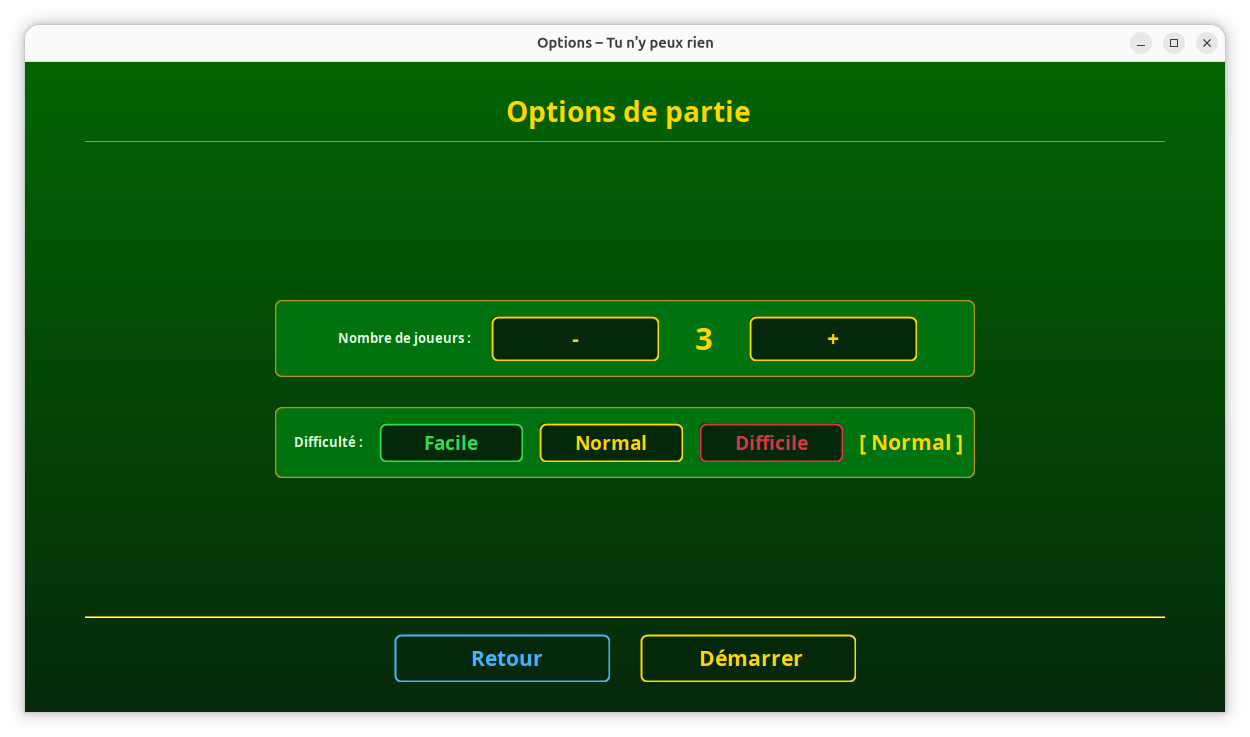
\includegraphics[width=10cm]{images/options.png}
\caption{Écran des options}
\label{fig:options}
\end{figure}

\subsection{Déroulement d'une partie}
\paragraph{} Le joueur humain est "Vous". Les bots sont représentés par des avatars. Pour jouer, sélectionnez des cartes dans votre main (clic gauche) puis cliquez sur "JOUER LES CARTES SÉLECTIONNÉES". Si vous ne pouvez pas jouer, cliquez sur "PIOCHER".

\begin{figure}[h!]
\centering
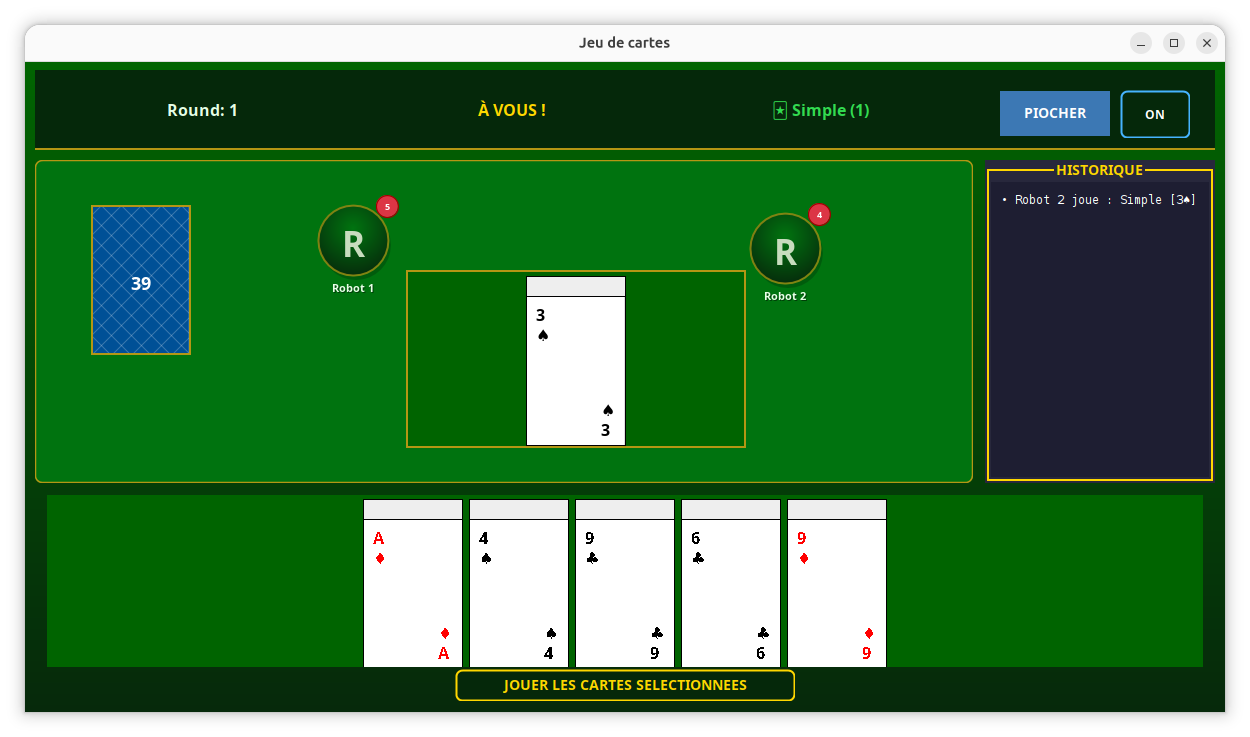
\includegraphics[width=12cm]{images/gameplay.png}
\caption{Interface de jeu}
\label{fig:gameplay}
\end{figure}

\subsection{Fin de partie}
\paragraph{} Quand un joueur n'a plus de cartes, l'écran de fin s'affiche avec le podium, les scores et les statistiques.

\begin{figure}[h!]
\centering
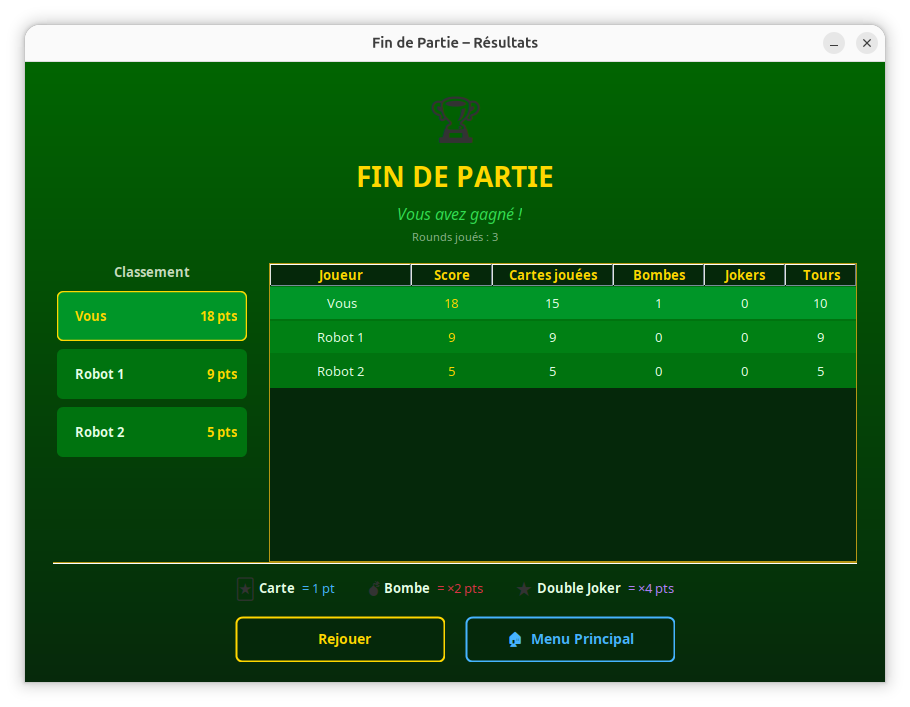
\includegraphics[width=12cm]{images/endgame.png}
\caption{Écran de fin de partie}
\label{fig:endgame}
\end{figure}

\newpage
\section{Déroulement du projet}
\label{sec:deroulement}

\subsection{Réalisation du projet par étapes}
\paragraph{} Le projet a été réalisé selon les étapes suivantes :

\begin{enumerate}
\item \textbf{Semaine 1-2} : Mise en place des classes de base (Card, Deck, Player)
\item \textbf{Semaine 3-4} : Implémentation des combinaisons (Combination, determineType, canBeat)
\item \textbf{Semaine 5-6} : Développement des bots et de la logique de jeu (Game)
\item \textbf{Semaine 7-8} : Interface graphique (Swing) et refonte du layout
\item \textbf{Semaine 9-10} : Tests unitaires (JUnit) et corrections de bugs
\item \textbf{Semaine 11-12} : Rédaction du rapport et préparation de la livraison
\end{enumerate}

\subsection{Répartition des tâches, communication et intégration}
\paragraph{} La répartition des tâches s'est organisée comme suit :

\begin{itemize}
\item \textbf{Laiza KHODJA} : Interface graphique (GameStyle, MusicPlayer, EndGameGUI, BotsPanel)
\item \textbf{Nesrine BOUATMANE} : Classes de données (Card, Deck, Player, GameStats, tests unitaires)
\item \textbf{Nassim BERRANDOU} : Logique métier (Game, Combination, bots, correction bugs)
\end{itemize}

\paragraph{} La communication s'est faite via Discord et GitHub. Le versionnement Git a permis une intégration continue des différentes parties.

\paragraph{} Les principaux défis rencontrés ont été :
\begin{itemize}
\item La gestion du reset du tas et du recyclage des cartes
\item La compatibilité de la musique entre Linux et Windows
\item La synchronisation des tours entre le joueur humain et les bots
\end{itemize}

\newpage
\section{Conclusion et perspectives}
\label{sec:conclusion}

\subsection{Résumé du travail réalisé}
\paragraph{} Le projet "Tu n'y peux rien" a été **mené à bien dans les délais impartis et a été entièrement achevé**. Toutes les fonctionnalités demandées dans le cahier des charges ont été implémentées et testées :

\begin{itemize}
\item Jeu complet avec interface graphique Swing fluide et responsive
\item 3 niveaux de difficulté pour les bots (Facile, Moyen, Difficile)
\item Détection robuste des combinaisons (simple, double, série, bombe, double joker)
\item Gestion correcte des cartes spéciales (2, Joker)
\item Système de scores et statistiques avec graphiques jFreeChart
\item Tests unitaires (JUnit) couvrant les classes critiques
\item Logs détaillés (Log4j) en HTML et texte
\end{itemize}

\paragraph{} Au total, ce sont **plus de 40 classes Java** qui ont été développées, pour environ **5000 lignes de code**. Le projet compile et s'exécute sans erreur sur les environnements cibles.

\subsection{Tests et validation}
\label{sec:tests}

\paragraph{} Les tests unitaires ont été réalisés avec JUnit 4. Chaque classe critique possède sa classe de test associée :

\begin{itemize}
\item \texttt{TestCard.java} : test de la création des cartes, des symboles et de l'égalité
\item \texttt{TestDeck.java} : test du mélange et de la pioche
\item \texttt{TestPlayer.java} : test de la pioche et de la pose de combinaisons
\item \texttt{TestCombination.java} : test de la détection des types et de la comparaison (15 cas)
\item \texttt{TestGameStats.java} : test du système de scores
\end{itemize}

\paragraph{} Au total, \textbf{37 tests unitaires} ont été écrits et passent tous avec succès. La couverture de code est satisfaisante sur les classes métier (\texttt{Combination}, \texttt{Player}, \texttt{GameStats}) mais reste partielle sur l'interface graphique (tests manuels uniquement).

\subsection{Améliorations possibles du projet}
\paragraph{} Bien que le projet soit fonctionnel et complet, plusieurs extensions pourraient enrichir l'expérience utilisateur :

\begin{itemize}
\item \textbf{Mode multijoueur en ligne} : Permettre à plusieurs joueurs humains de jouer à distance via réseau (sockets Java)
\item \textbf{Sauvegarde des parties} : Sauvegarder l'état du jeu dans un fichier pour le reprendre plus tard
\item \textbf{Classements et statistiques persistants} : Stocker les scores et victoires dans une base de données SQLite
\item \textbf{Animations} : Ajouter des animations lors de la pose des cartes (transition, mouvement)
\item \textbf{Thèmes personnalisables} : Permettre au joueur de changer l'apparence des cartes et du tapis (plusieurs skins)
\item \textbf{Version mobile} : Adapter le jeu pour Android via un wrapper ou une réécriture partielle
\end{itemize}

\paragraph{} En conclusion, le projet "Tu n'y peux rien" remplit l'ensemble des objectifs fixés. Il démontre la maîtrise des concepts de génie logiciel (Java, Swing, patterns, tests, Git) et offre une expérience de jeu complète et agréable. Ces améliorations constitueraient une excellente base pour une version 2.0 du projet.

\newpage
\section{Annexes}
\label{sec:annexes}

\subsection{Guide d'installation rapide}
\paragraph{Prérequis :}
\begin{itemize}
\item Java 8 ou supérieur (JDK 1.8+)
\item Eclipse IDE (version 2020-06 ou supérieure)
\end{itemize}

\paragraph{Import du projet dans Eclipse :}
\begin{enumerate}
\item Ouvrir Eclipse
\item \texttt{File $\rightarrow$ Import $\rightarrow$ Git $\rightarrow$ Projects from Git}
\item Sélectionner \texttt{Clone URI}
\item Renseigner : \texttt{https://github.com/berrandou-dev/Projet\_GLP-Jeu\_Carte.git}
\item Suivre les instructions par défaut
\item Une fois importé, faire \texttt{Project $\rightarrow$ Clean} pour forcer la compilation
\end{enumerate}

\paragraph{Ajout des bibliothèques externes :}
\begin{enumerate}
\item Faire clic droit sur le projet $\rightarrow$ \texttt{Build Path $\rightarrow$ Configure Build Path}
\item Onglet \texttt{Libraries} $\rightarrow$ \texttt{Add JARs...}
\item Sélectionner tous les JARs dans \texttt{src/lib/} :
\begin{verbatim}
- log4j-1.2.17.jar
- junit-4.11.jar
- jfreechart-1.0.19.jar
- jcommon-1.0.23.jar
\end{verbatim}
\item Cliquer sur \texttt{Apply and Close}
\end{enumerate}

\paragraph{Lancement du jeu :}
\begin{enumerate}
\item Dans l'Explorateur de projet, naviguer vers \texttt{src/test/manual/}
\item Faire clic droit sur \texttt{TestGame.java} $\rightarrow$ \texttt{Run As $\rightarrow$ Java Application}
\item Le menu principal apparaît
\end{enumerate}

\subsection{Structure des packages du projet}
\paragraph{} Le projet est organisé selon l'architecture MVC :

\begin{verbatim}
src/
+-- config/           # Configuration (GameConfig.java)
+-- engine/
    +-- data/         # MODELE : Card, Deck, Player, GameStats
    +-- process/      # CONTROLEUR : Game, Combination, bots
+-- gui/
    +-- panels/       # VUE : composants reutilisables
    +-- screens/      # VUE : ecrans complets
    +-- utils/        # Utilitaires : GameStyle, MusicPlayer, ChartManager
+-- lib/              # Bibliotheques externes (JARs)
+-- log/              # Logs generes (ignores par Git)
+-- resources/        # Images et musique
+-- test/             # Tests unitaires (JUnit)
    +-- demo/         # Mode demonstration
    +-- manual/       # Tests manuels (TestGame, TestEndGameGUI)
    +-- unit/         # Tests unitaires par classe
\end{verbatim}

\subsection{Principales classes du projet}
\paragraph{} Voici un résumé des classes les plus importantes :

\begin{table}[h!]
\centering
\begin{tabular}{|l|l|p{6cm}|}
\hline
\textbf{Classe} & \textbf{Package} & \textbf{Rôle} \\
\hline
\texttt{Card} & engine.data & Représente une carte (valeur + couleur) \\
\texttt{Deck} & engine.data & Gère le paquet de 54 cartes \\
\texttt{Player} & engine.data & Gère la main du joueur \\
\texttt{GameStats} & engine.data & Enregistre les scores et statistiques \\
\hline
\texttt{Game} & engine.process & Logique principale du jeu \\
\texttt{Combination} & engine.process & Détection et comparaison des combinaisons \\
\texttt{BotPlayer} & engine.process & Classe abstraite pour les bots \\
\hline
\texttt{MainGUI} & gui.screens & Interface principale du jeu \\
\texttt{EndGameGUI} & gui.screens & Écran de fin de partie avec graphiques \\
\texttt{ChartManager} & gui.utils & Génération des graphiques jFreeChart \\
\hline
\end{tabular}
\caption{Principales classes du projet}
\label{tab:classes}
\end{table}


\newpage
%Références bibliographiques du document
\bibliographystyle{plain}
\bibliography{bibliographies}
\nocite{*}

\end{document}
